% this file is called up by thesis.tex
% content in this file will be fed into the main document

\chapter{Replacement for Hit Correlation Step} % top level followed by
% section, subsection
\label{cha:mlp}

% ----------------------- contents from here ------------------------
% 
This chapter presents the replacement created using a Multi Layered
Perceptron (MLP) for the \textit{Hit Correlation Step} of the Karas
pipeline (see \ref{cha:karas-pipeline}). It is observed that a MLP is
able to identify causally related hits with a higher accuracy,
precision and recall compared to the PMC. The chapter begins by
explaining how the data is created followed by its visual examination.
The training and testing procedure for the model is explained next.
The chapter concludes with discussions of the experiment results and
next steps.

\section{Data Preparation}
\label{sec:mlp-data-prep}

Figure \ref{fig:mlp-data} summarizes the MLP dataset creation process.
With an input data of shape $(n, 4)$ (\emph{n} rows and 4 columns
representing \emph{x, y, z, and t}), an output data of shape
\texttt{($\sum_{k=n-1}^{1}k$, 9)} is obtained. A significant rise in
the number of rows is observed since each row (representing a single
hit) is paired with all rows that follow. The output dataset consists
of 9 columns due to the presence of \emph{x, y, z and t} columns of
two hits plus the label column.

\begin{figure}[htb]
  \centering
  \begin{minipage}[t]{0.74\textwidth}
    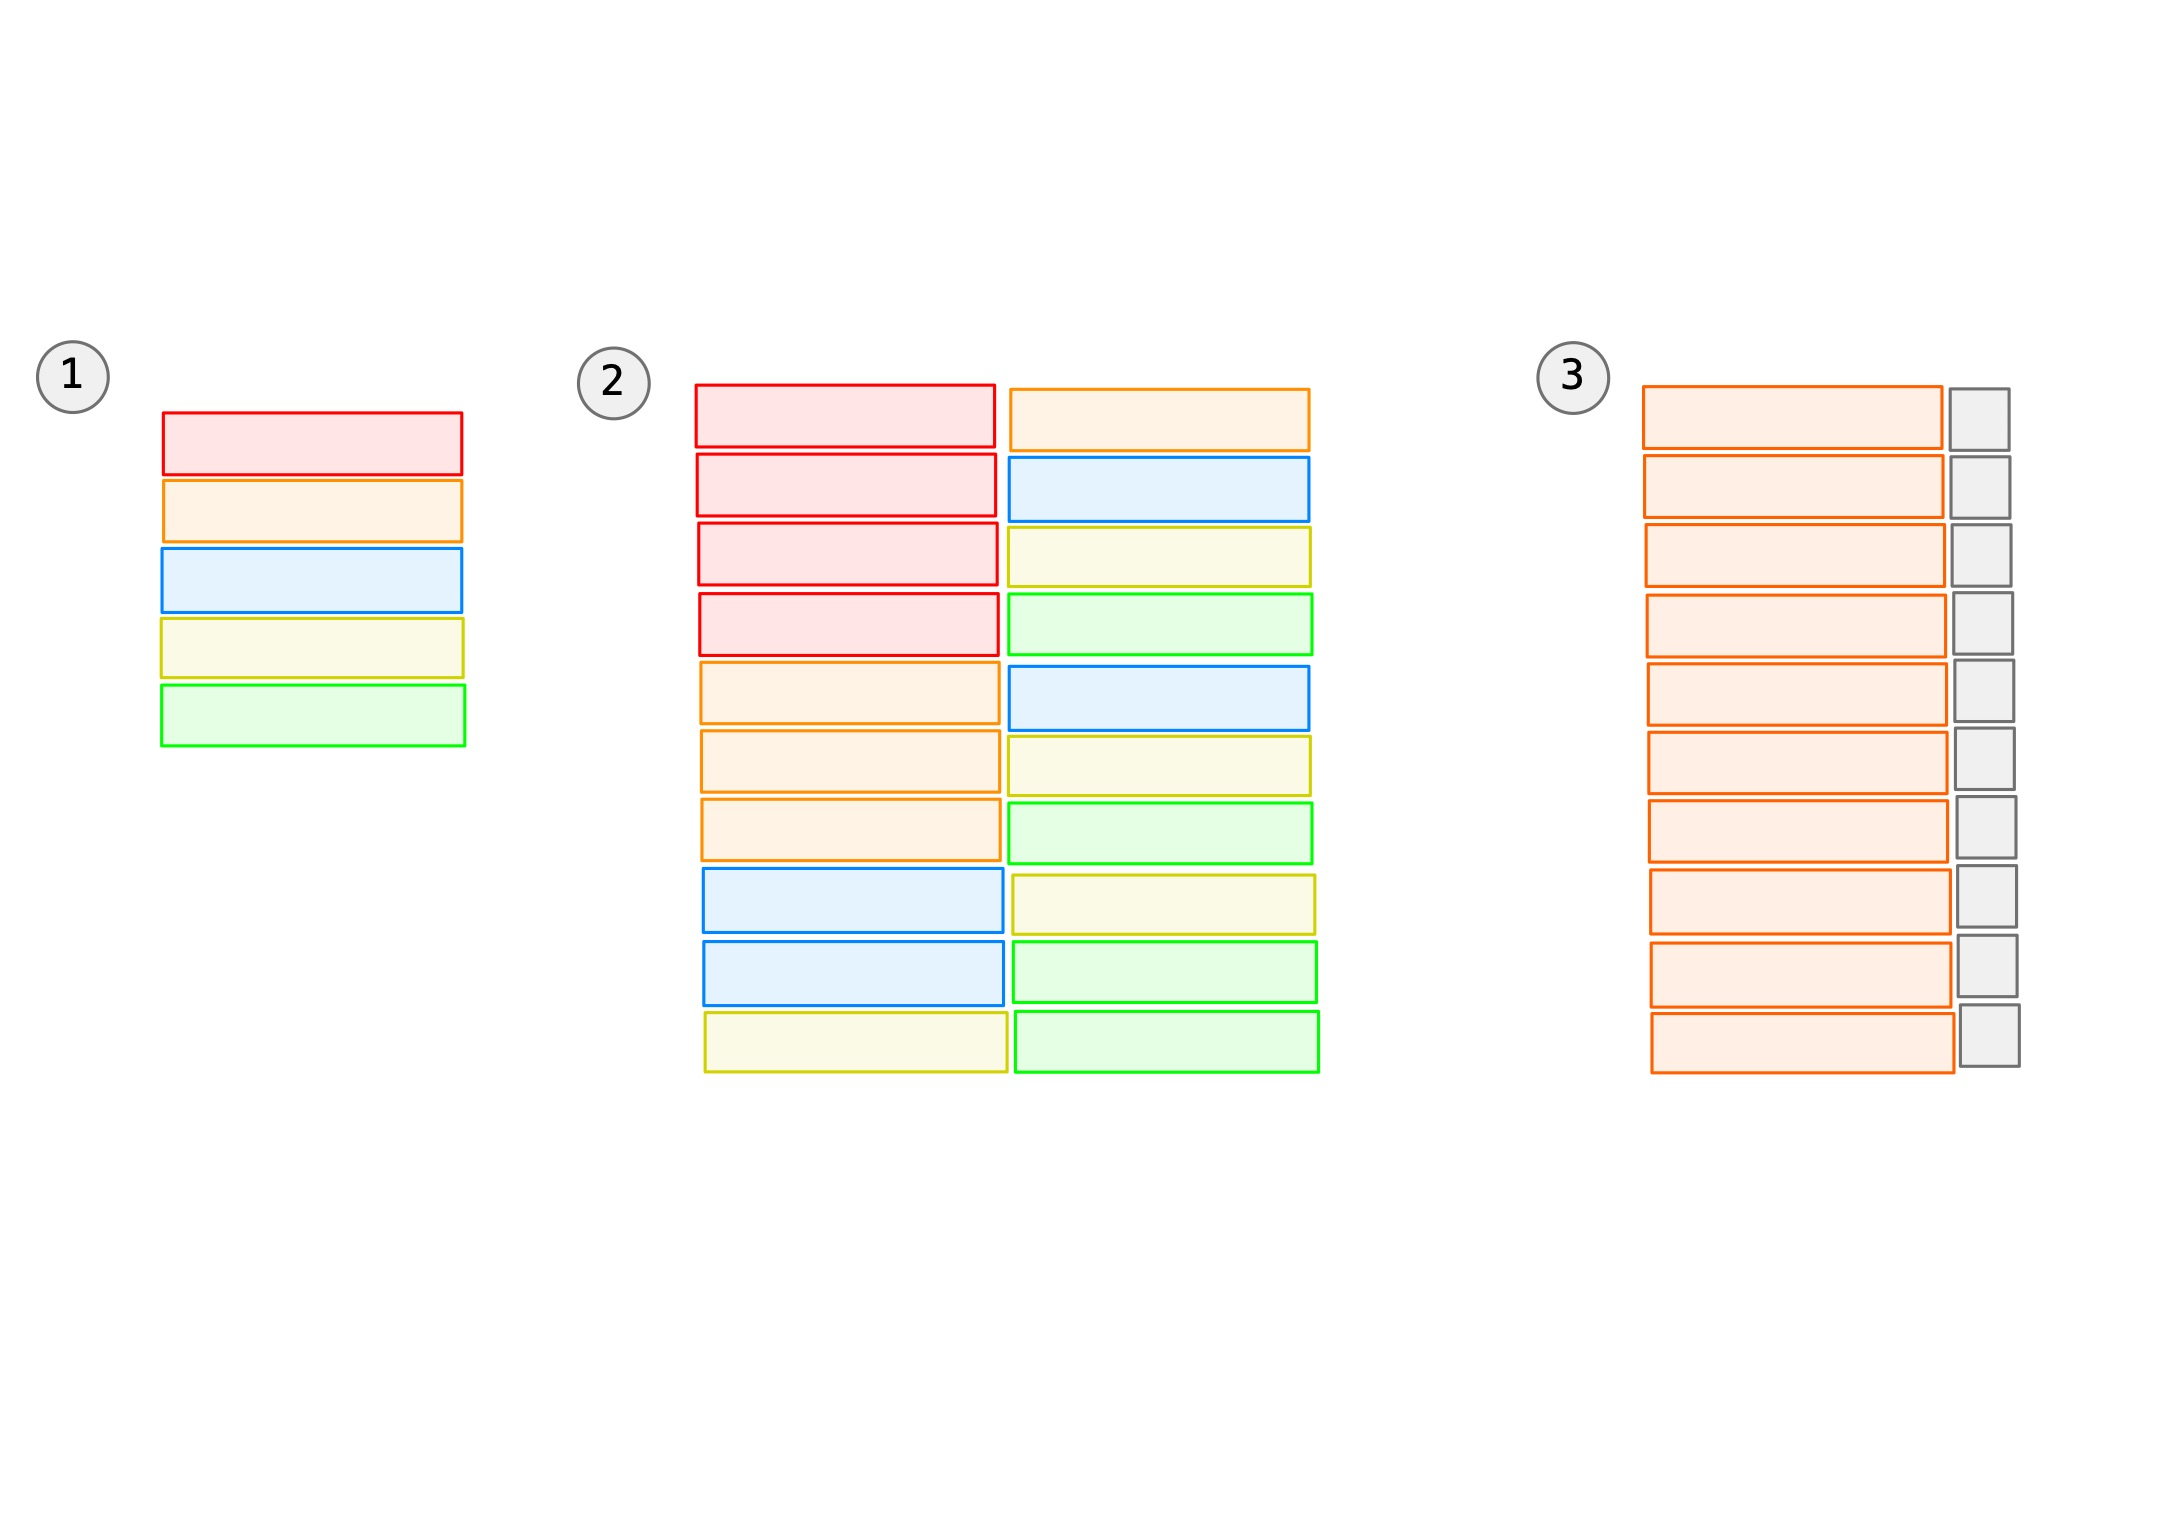
\includegraphics[width=\textwidth]{mlp-data.jpg}
    \caption{Overview of MLP dataset creation procedure. \textbf{(1)}
      The main dataset where each row represents a hit, here an example
      set containing 5 rows is shown for simplicity. \textbf{(2)} The
      MLP dataset is generated from the main dataset consisting of all
      unique pairs of hits. Algorithmically, this is done by pairing
      each hit with the subsequent hits below it as demonstrated with
      the use of colors. \textbf{(3)} The difference between the hits is
      taken (dark orange) and a label is assigned to each row (gray).}
    \label{fig:mlp-data}
  \end{minipage}
  \begin{minipage}[t]{0.24\textwidth}
    \centering
    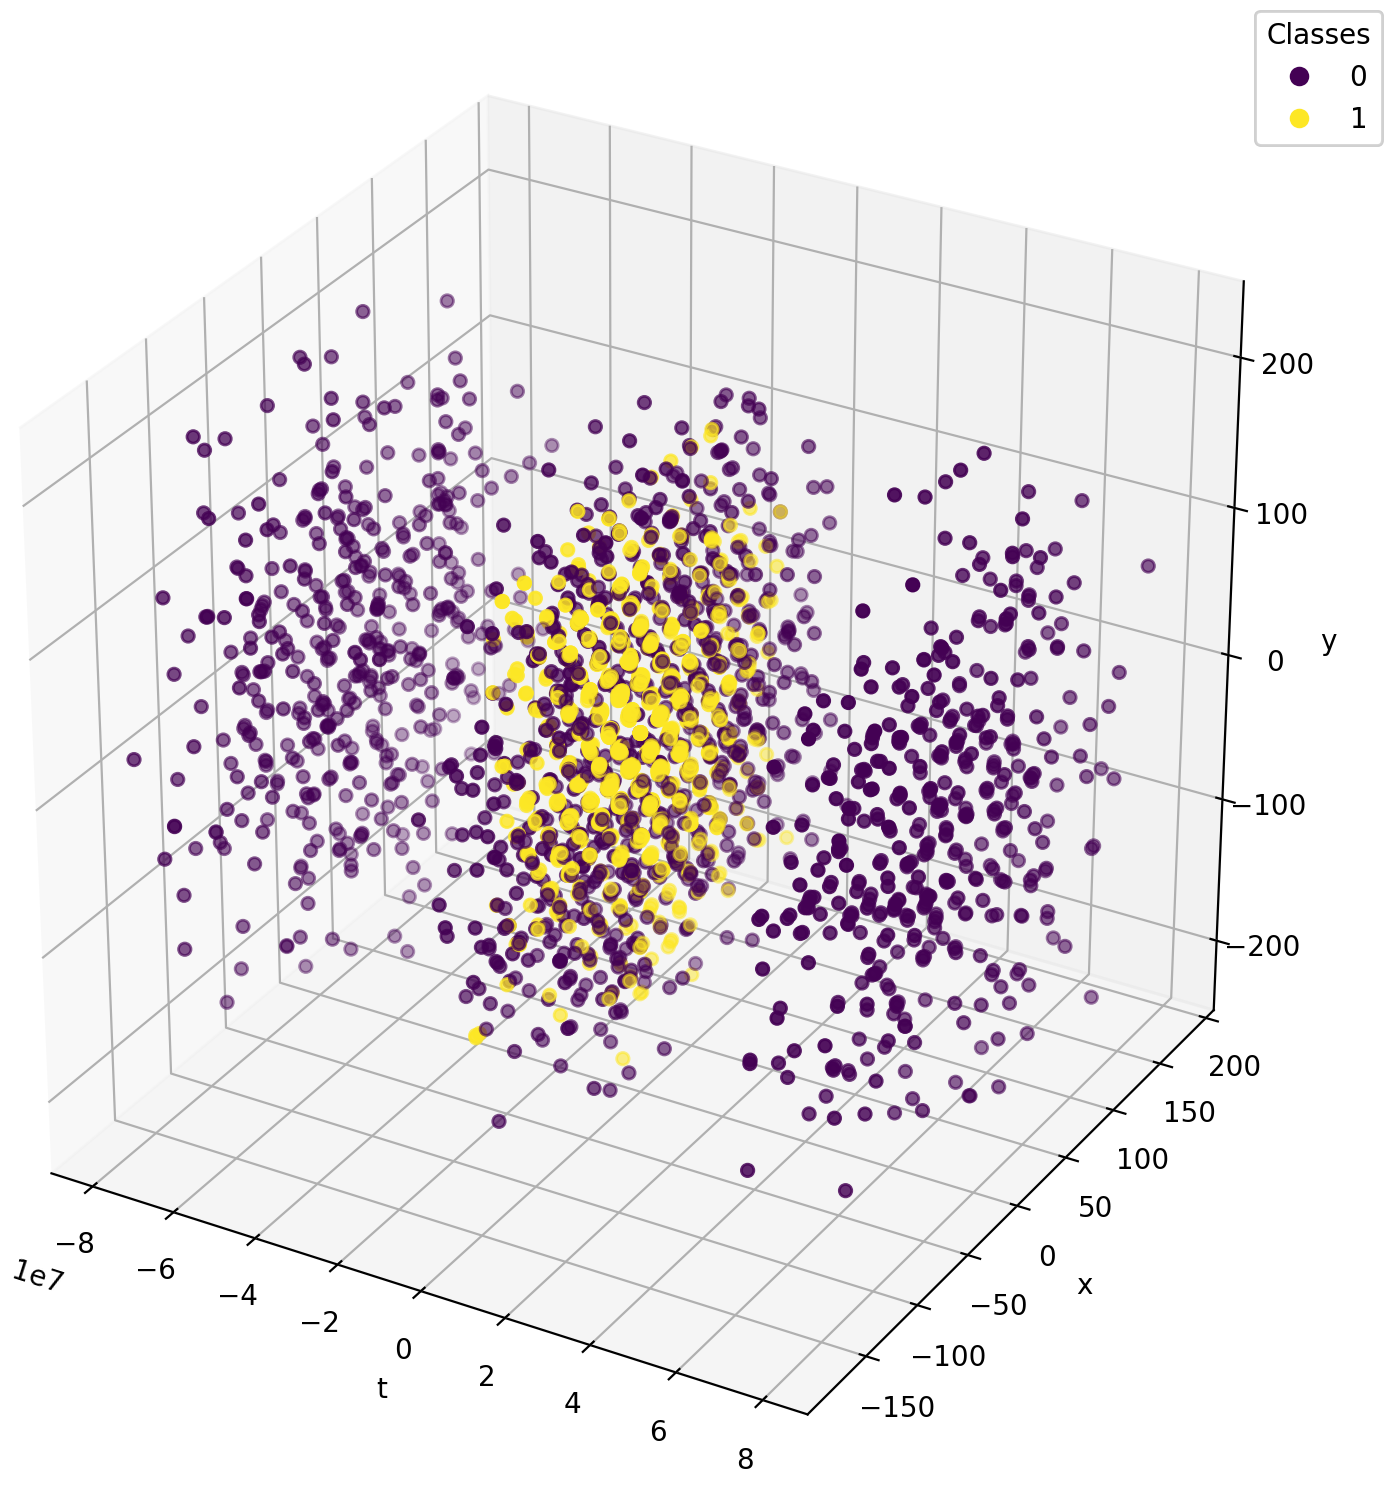
\includegraphics[width=\linewidth]{mlp-train-dist.png}
    \caption{Distribution of MLP training dataset.}
    \label{fig:mlp-train-dist}
  \end{minipage}
\end{figure}

The label column is populated based on the values of the
\texttt{event\_id} column of the two hits. The row is assigned a label
of 1 if the two hits have the same event id, which signifies that they
originated from the same neutrino event and hence are causally related
to each other. If the event id of the two hits are not the same then
they are assigned a label of 0.

Better model performance was observed when the model was trained with
the difference between hits in time and space. As a result, the final
dataset of shape \texttt{$\sum_{k=n-1}^{1}k$, 5} was obtained. The
fist 4 columns being the difference of \emph{x, y, z and t} vectors of
the paired hits and the last column being the label. The data is
additionally scaled between $[0,1]$ as this is recommended and
empirically proven to improve model performance and prevent vanishing
gradients during training
\cite{bengio2012practical,goodfellow-et-al-2016}.

\subsection{Preparation of Training Data}
\label{sec:mlp-data-prep-train}

The main dataset is highly skewed, with the \textbf{majority or
  negative class} being hits from background noise and the
\textbf{minority or positive class} being hits from neutrino events.
Thus, the training set created is also skewed with the minority class
being related hits and majority class being unrelated hits. To
maximize the number of positive examples in the training set, a random
sample was taken from the top 5 timeslices of the main dataset with
the most number of event hits. The model is required to classify
related and unrelated hits which can be done by observing the space
and time difference between the given points. Since this phenomenon is
consistent across the entire main dataset, training using a sample
does not introduce any bias into the model.

The training set still however contains a skewed distribution of
examples, and training the model with such a dataset will result in a
model that is biased to the majority class. To combat this problem,
the majority class is \emph{undersampled} such that the number of
examples for each class is the same. Figure \ref{fig:mlp-train-dist}
shows the distribution of a random sample of the training set. It is
observed that the related hits occur close to one another in space and
time whilst the noise hits are scattered throughout which should aid
the model to learn. A fraction of the training set is kept as a hold
out or validation set to evaluate the model's training. Table
\ref{tab:mlp-train-dist} presents the distribution of the training and
validation sets.

\begin{table}[htb]
  \centering
  \caption{Distribution of MLP Training and Validation Datasets.}
  \begin{tabular}{lrrr}
    \hline
    & Total examples & Positive examples & Negative examples \\
    Training & 48,434 & 24,217 & 24,217 \\
    Validation & 23,856 & 11,928 & 11,928 \\
    \hline
  \end{tabular}
  \label{tab:mlp-train-dist}  
\end{table}

\subsection{Preparation of Testing Data}
\label{sec:mlp-data-prep-test}

Whilst the training dataset contains equal number of examples for each
class, the testing dataset maintains it's skewed distribution since
this represents realistic data which the model will be required to
classify. Four variants of the testing dataset with varying level of
examples of related hits were created as listed in Table
\ref{tab:mlp-test-dist}. In practice, the pipeline will observe
timeslices which contain no to very few related hits, thus the
performance of the model on TS1 and TS2 are of vital importance.

\begin{table}[htb]
  \centering
  \caption{Distribution of MLP Test Datasets.}
  \begin{tabular}{lrrr}
    \hline
    & Total examples & Positive examples & Negative examples \\
    \textbf{TS1} & 774,390 & -- & 774,390 \\
    \textbf{TS2} & 5,829,405 & 10 & 5,829,395 \\
    \textbf{TS3} & 5,880,735 & 1176 & 5,879,559 \\
    \textbf{TS4} & 364,231 & 8,372 & 355,859 \\
    \hline
  \end{tabular}
  \label{tab:mlp-test-dist}
\end{table}

\section{Model Description}
\label{sec:mlp-model-desc}

The expectation of the model is to identify if two given points are
causally related to each other or not. As revealed through data
exploration in Chapter \ref{cha:data-exploration}, hits originating from
neutrino events occur close to each other in space and time. Thus, The
expectation from the model is to learn this phenomenon by training
over pairs of points and classify unseen data as related or unrelated.

\begin{table}[htb]
  \centering
  \begin{tabular}{lr}
    \hline
    Loss & BCELoss \\
    Optimizer & Adam \\
    Learning rate & 0.001 \\
    Hidden activation function & ReLU\\
    Output activation function & Sigmoid \\
    Training batch size & 16 \\
    Testing batch size & 32 \\
    \hline
  \end{tabular}
  \caption{GCN Model Parameter Summary.}
  \label{tab:gcn-model-param}
\end{table}

The parameters of the model are summarized in Table
\ref{tab:mlp-model-param}. The Adam optimizer with a learning rate of
$0.001$ is used to optimize the loss function since it is considered a
reasonable start for many optimization problems and has been
empirically proven to outperform other algorithms such as
\textit{Stocastic Gradient Descent (SGD)}, \textit{RMSProp} and
\textit{Adagrad} \cite{ruder2016overview}. Being a binary
classification task, the \textit{Binary Cross Entropy Loss (BCELoss)}
(also known as \textit{Log Loss}) was selected as the loss function
since it has been established as the standard loss function for binary
classification tasks \cite{painsky2018universality}. As the BCELoss
function expects an input in the range of $[0, 1]$, the
\textit{Sigmoid} activation function was chosen for the output layer.
The \textit{ReLU} activation function was chosen for the hidden layers
since it is generally considered a good start for most problems
\cite{nwankpa2018activation, wang2019learning}. A batch size of 16 is
used for the training and validation sets whilst a larger batch size
of 32 is used for the testing set since these value are often
recommended as good defaults by machine learning practitioners
\cite{bengio2012practical,Goodfellow-et-al-2016}.

\begin{table}[htb]
  \centering
  \begin{tabular}{lrrrr}
    \hline
    Layer Position & Type & Activation & In features & Out features \\
    1 & Linear & ReLu & 4 & 16 \\
    2 & Linear & ReLU & 16 & 8 \\
    3 & Linear & Sigmoid & 8 & 1 \\
    \hline
  \end{tabular}
  \caption{MLP Model Architecture Summary.}
  \label{tab:mlp-model-arch}
\end{table}

The model architecture is summarized in Table
\ref{tab:mlp-model-arch}. It consists of an input layer, two hidden
layers and an output layer. The network is fully connected with 4
neurons in the input layer, 16 neurons in the first hidden layer, 8 in
the second hidden layer and finally 1 neuron in the output layer. The
optimal value of all parameters stated above were identified either
empirically or from recommendations presented in literature. The
number of epochs used to train the model is not mentioned above since
this parameter is largely determined by the dataset, batch size and
the learning rate, thus its value varied per experiment.

\section{Model Evaluation}
\label{sec:mlp-model-eval}

The model is evaluated using several metrics which are regarded as the
standard set of metrics to evaluate machine learning model.
Additionally, metrics geared towards evaluating a model performing
binary classification on skewed datasets are considered as well.

\begin{enumerate}
\item \textbf{Accuracy}. The accuracy is the ability of a model to
  classify unseen data correctly and is mathematically defined by
  Equation \ref{eq:accuracy}.

  \begin{equation}
    Accuracy = \frac{Number of correct predictions}{Total number of examples}
    \label{eq:accuracy}
  \end{equation}
  
\item \textbf{Learning Curve}. The Learning curve is a line plot of
  the loss over the training epochs. A model with a good fit results
  in a loss curve which approaches 0 with time.
  
\item \textbf{Confusion Matrix (CM)}. For highly skewed data, accuracy
  is not a good metric for evaluating the model performance
  \cite{branco2015survey} since it may achieve a high score by simply
  predicting the majority class. Thus the CM is used to visualize the
  number of \emph {true positive (TP)}, \emph{true negative (TN)},
  \emph{false positive (FP)} and \emph{false negative (FN)}
  predictions of the model.
\item \textbf{Recall}. The recall is the ability of the model to
  correctly identify the minority class. For this problem, the recall
  of the model is given precedence over its precision. This is because
  the model should be able to identify all instances of the positive
  class since this determines if the timeslice will ultimately be
  saved or not. The recall is mathematically defined by Equation
  \ref{eq:recall}.

  \begin{equation}
    \frac{TP}{TP + FN}
    \label{eq:recall}
  \end{equation}

\item \textbf{Precision}. The precision is the ability of the model to
  not misclassify an instance of the negative class (ie. classify it
  as the positive class). Although this should also be high, it is
  often inversely proportional to recall. The precision is
  mathematically defined by Equation \ref{eq:precision}.

  \begin{equation}
    \frac{TP}{TP + FP}
    \label{eq:precision}
  \end{equation}

\item \textbf{F1 score}. The F1 score is the harmonic mean of the
  precision and recall, thus it is a single metric to summarize the
  model's performance based on its precision and recall. The F1 score
  is a value between $[0, 1]$ with a value close to 1 indicating high
  precision and recall. The F1 score is mathematically defined by
  Equation \ref{eq:f1-score}.

  \begin{equation}
    \frac{2 * (Precision * Recall)}{Precision + Recall}
    \label{eq:f1-score}
  \end{equation}
  
\item \textbf{F2 score}. Since recall is given precedence for this
  problem, the F2 score can be considered a better alternative to the
  F1 score as it gives higher importance to the recall through the
  $\beta$ parameter. The F2 score is mathematically defined by
  Equation \ref{eq:f2-score}. Thus the F2 score with $\beta = 1$ is
  equivalent to the F1 score.

  \begin{equation}
    \frac{(1 + \beta^{2}) * Precision * Recall}{(\beta^{2}) *
      (Precision + Recall)}
    \label{eq:f2-score}
  \end{equation}
  
\item \textbf{Receiver Operating Characteristic (ROC) curve} is a plot
  of the \emph{true positive rate (TPR)} and the \emph{false positive
  rate (FPR)} (mathematically defined by Equations \ref{eq:tpr-fpr})
  across various discrimination probability thresholds of the model.
  The ROC curve can be interpreted as the fraction of correct
  predictions for the positive class (along the y-axis) versus the
  fraction of error in predictions for the negative class (along the
  x-axis). The area under the ROC curve (ROCAUC) can be used to
  summarize the ROC curve with a singular value. Thus, a highly
  skilled model has a ROC curve which arches from $(0,0)$ to $(1,1)$
  with a ROCAUC  between 0.5 and 1.0. Whilst the ROC curve of a model
  without any skill is a straight line from $(0,0)$ to $(1,1)$ with a
  ROCAUC of 0.5.


  \begin{equation}
    TPR = \frac{TP}{TP + FN}
    FPR = \frac{FP}{FP + TN}
    \label{eq:tpr-fpr}
  \end{equation}
  
\item \textbf{Precision-Recall (PR) Curve} can be considered a better
  alternative to the ROC curve since the ROC curve can be overly
  optimistic of the model's skill when dealing with highly skewed data
  since it considers the model's performance for both the classes. In
  contrast, the PR curve is a diagnostic plot of the model's precision
  and recall across various discrimination probability thresholds of
  the model. Thus the PR curve only considers the model's performance
  with regards to the positive class. Similar to the ROC curve, the PR
  curve can also be summarized by the area under the curve or the
  PRAUC. A skilled model, thus has a PR curve which bows towards
  $(1,1)$ whilst a model with no skill is a horizontal line.
\end{enumerate}

\section{Results}
\label{sec:mlp-disc}

%% TODO limitation: due to stocastic nature of hits, mlp is unable to
%% solve the problem of truly unrelated hits being classified as related
%% hits. This is the reason why performance of the model decreases as we
%% increase the number of event hits (TS4)

Figure \ref{fig:mlp-learning} shows the learning curve of the model on
the training and validation tests. The curves approach zero with time
and remain in close proximity to each other indicating a good fit.
Table \ref{tab:mlp-results} summarizes the model's performance across
the various test sets (see Section \ref{sec:mlp-data-prep-test}). In
general, the model performs well with high accuracy and recall across
all test sets. The model achieves almost perfect recall for TS2 and
TS3 which have extremely low positive examples which speaks to its
strength. The poor precision scores can be attributed to the skewed
nature of the datasets. Since the FPs are relatively high compared to
the TPs in the datasets, the precision falls drastically. This is also
corroborated by the fact that the recall in TS4 increases due to a
better FP:TP ratio (see Figure \ref{fig:mlp-cm}).

\begin{figure}[htb]
  \centering
  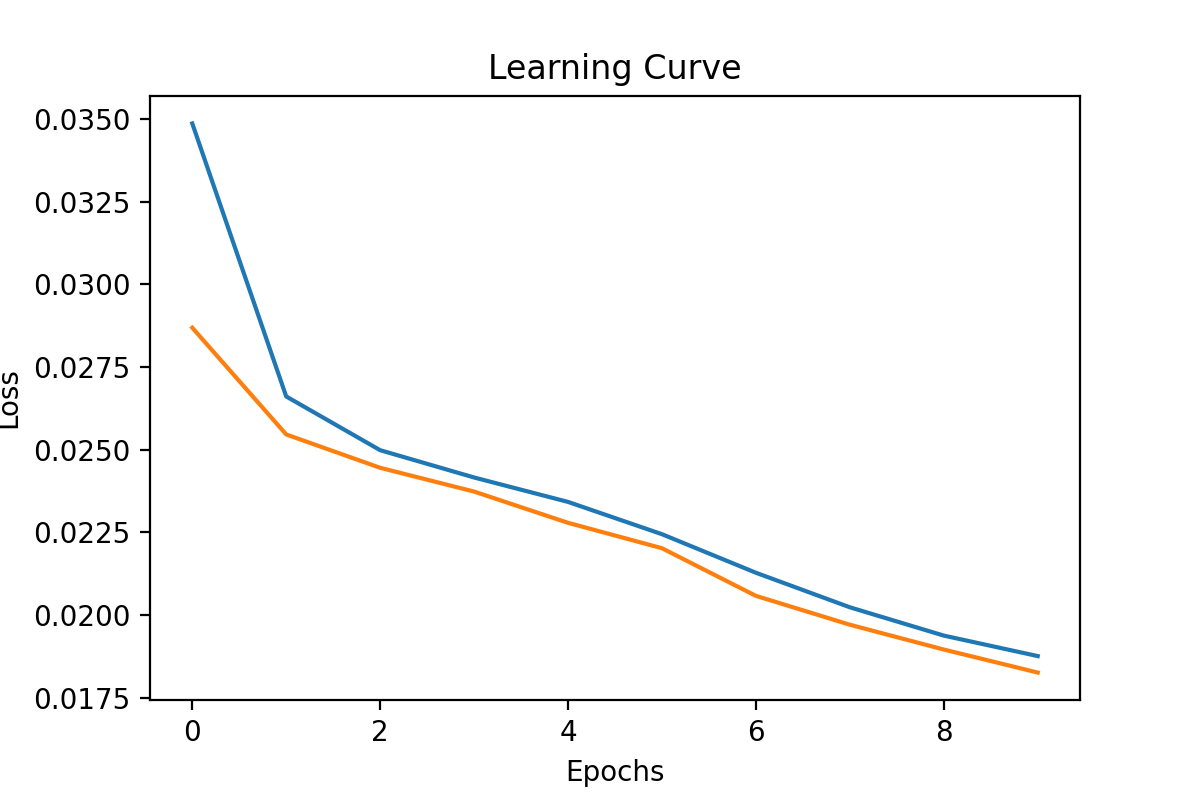
\includegraphics[width=0.5\textwidth]{mlp-learning.png}
  \caption{Learning Curve of MLP Training and Validation Datasets.}
  \label{fig:mlp-learning}
\end{figure}

\begin{table}[htb]
    \centering
    \begin{tabular}{rrrrrrrr}
      \hline
      & Accuracy & Precision & Recall & F1 & F2 & ROCAUC & PRAUC \\
      TS1 & 0.80 & -- & -- & -- & -- & -- & -- \\
      TS2 & 0.91 & 0.00 & 1.00 & 0.00 & 0.00 & 0.99 & 0.00 \\
      TS3 & 0.92 & 0.00 & 0.98 & 0.00 & 0.01 & 0.98 & 0.01 \\
      TS4 & 0.92 & 0.19 & 0.83 & 0.31 & 0.48 & 0.96 & 0.33 \\
      \hline
    \end{tabular}
    \caption{Summary of MLP performance across test sets.}
    \label{tab:mlp-results}
\end{table}

\begin{figure}[htb]
  \centering
  \begin{minipage}{0.32\textwidth}
    \centering
    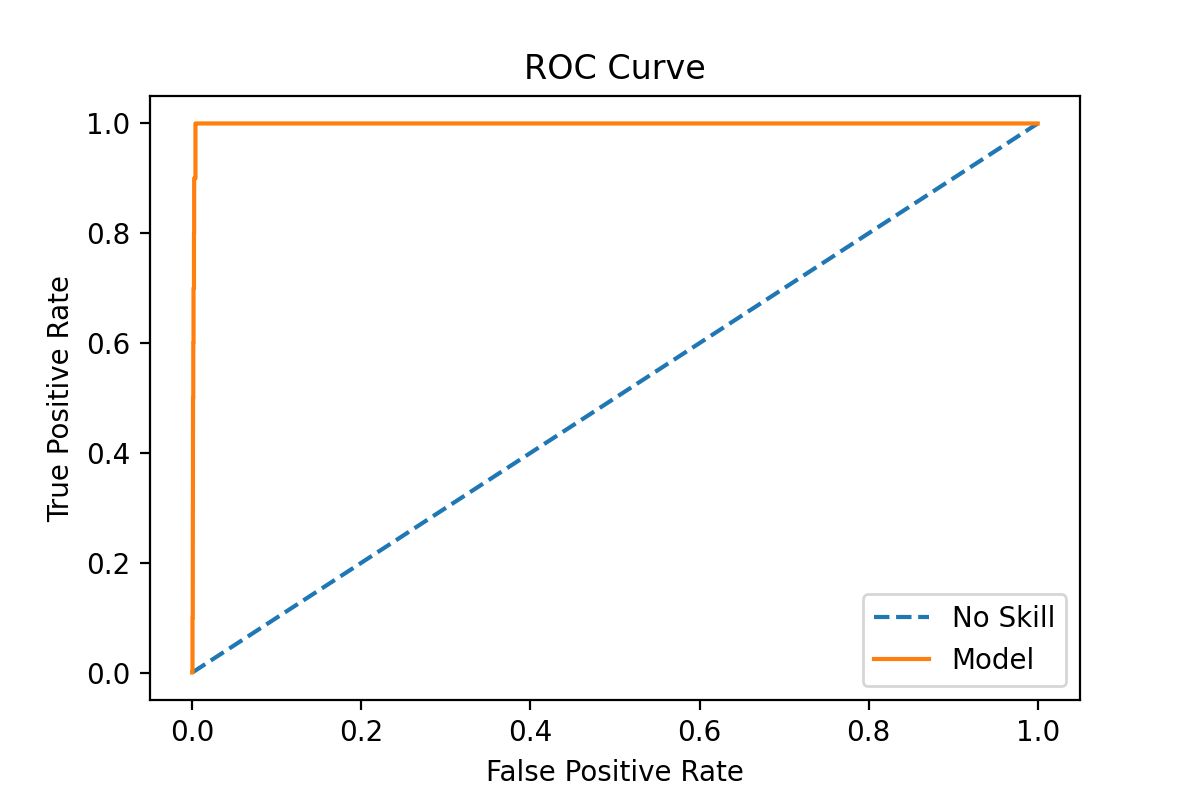
\includegraphics[width=\linewidth]{mlp-roc-low.png}
    \caption{ROC Curve for TS2.}
  \end{minipage}
  \begin{minipage}{0.32\textwidth}
    \centering
    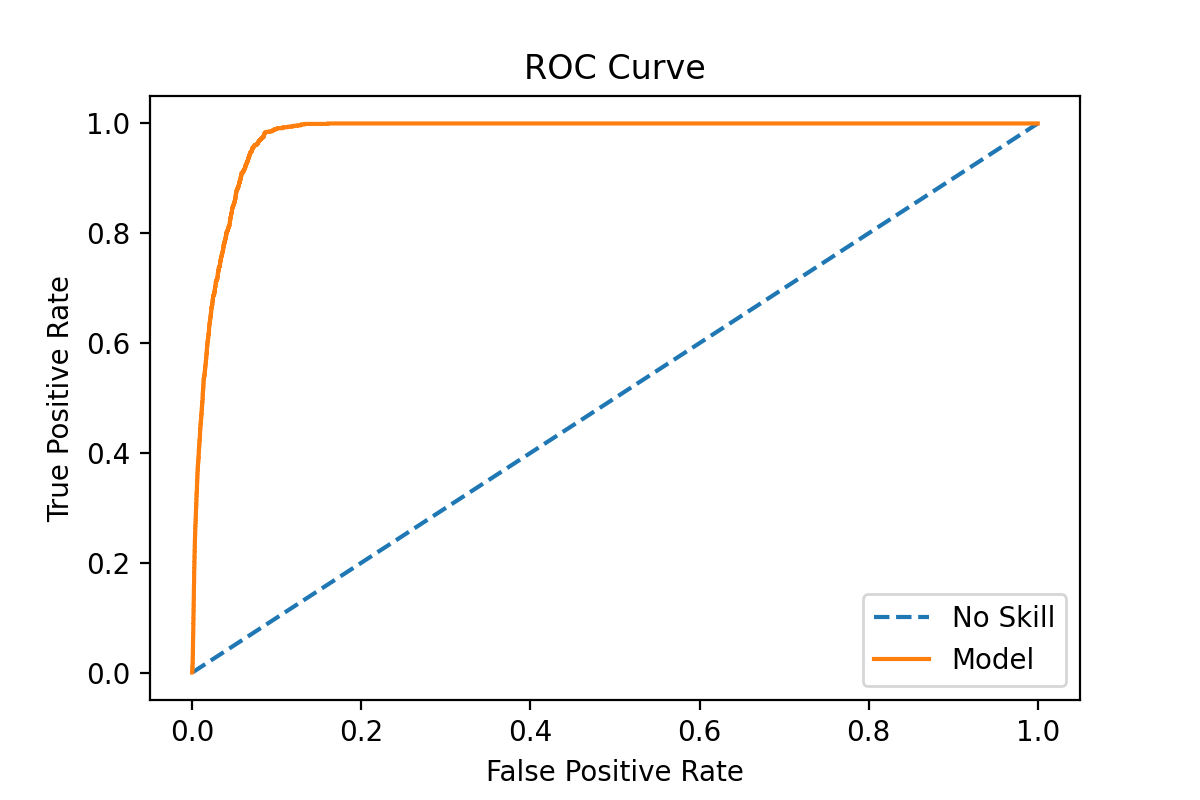
\includegraphics[width=\linewidth]{mlp-roc-medium.png}
    \caption{ROC Curve for TS3.}
  \end{minipage}
  \begin{minipage}{0.32\textwidth}
    \centering
    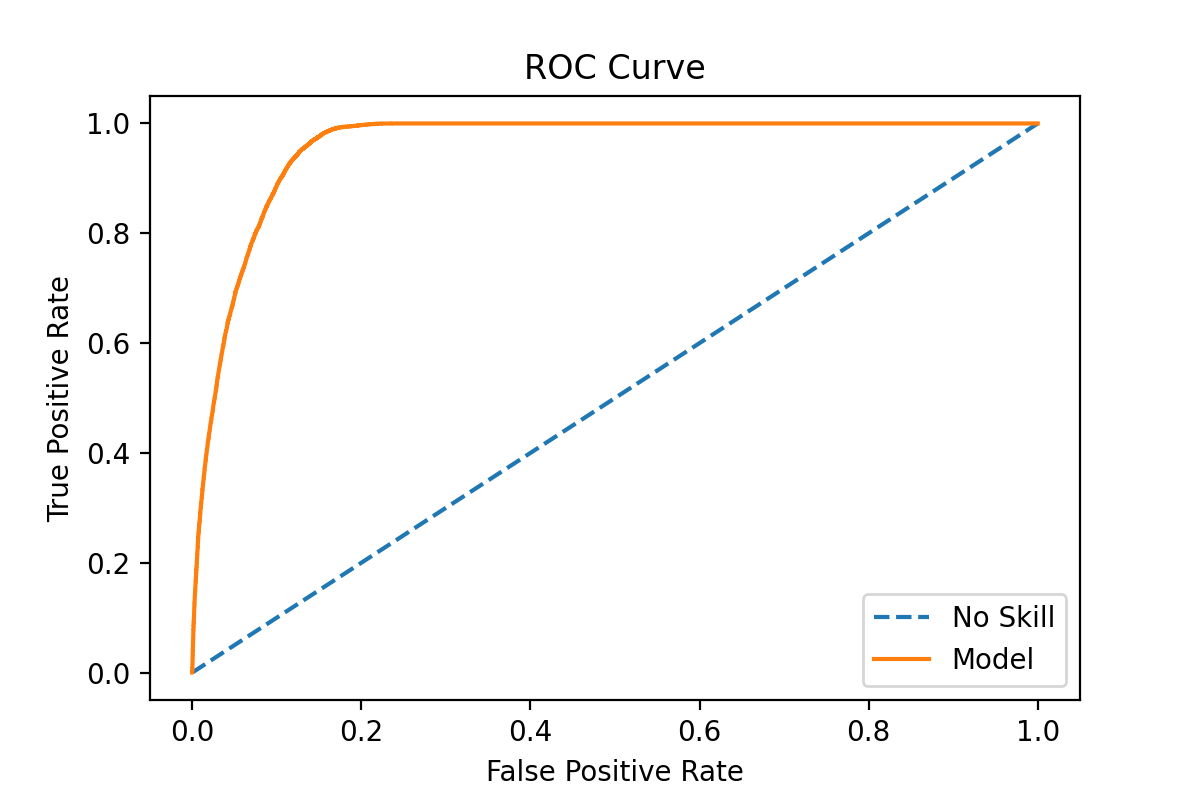
\includegraphics[width=\linewidth]{mlp-roc-high.png}
    \caption{ROC Curve for TS4.}
  \end{minipage}
  \caption{ROC Curves for MLP Test Datasets.}
  \label{fig:mlp-roc}
\end{figure}

The ROC curves paint a different picture (see Figure
\ref{fig:mlp-roc}) with exceedingly high areas. This however is
misleading since ROC curve takes into account the performance for both
the positive and negative classes and thus tend to be overly
optimistic of the model's performance on skewed datasets
\cite{branco2015survey,fernandez2018learning}. In such circumstances,
The PR curves are considered better at gauging a model's skill when
dealing with skewed datasets \cite{branco2015survey}. However, in this
case it too is deemed misleading as it seriously undermines the
model's performance (see Figure \ref{fig:mlp-pr}). This again is
attributed to the precision approaching zero due to the extremely
skewed FP:TP ratio which results in the PRAUC to also be zero.

\begin{figure}[htb]
  \centering
  \begin{minipage}{0.32\textwidth}
    \centering
    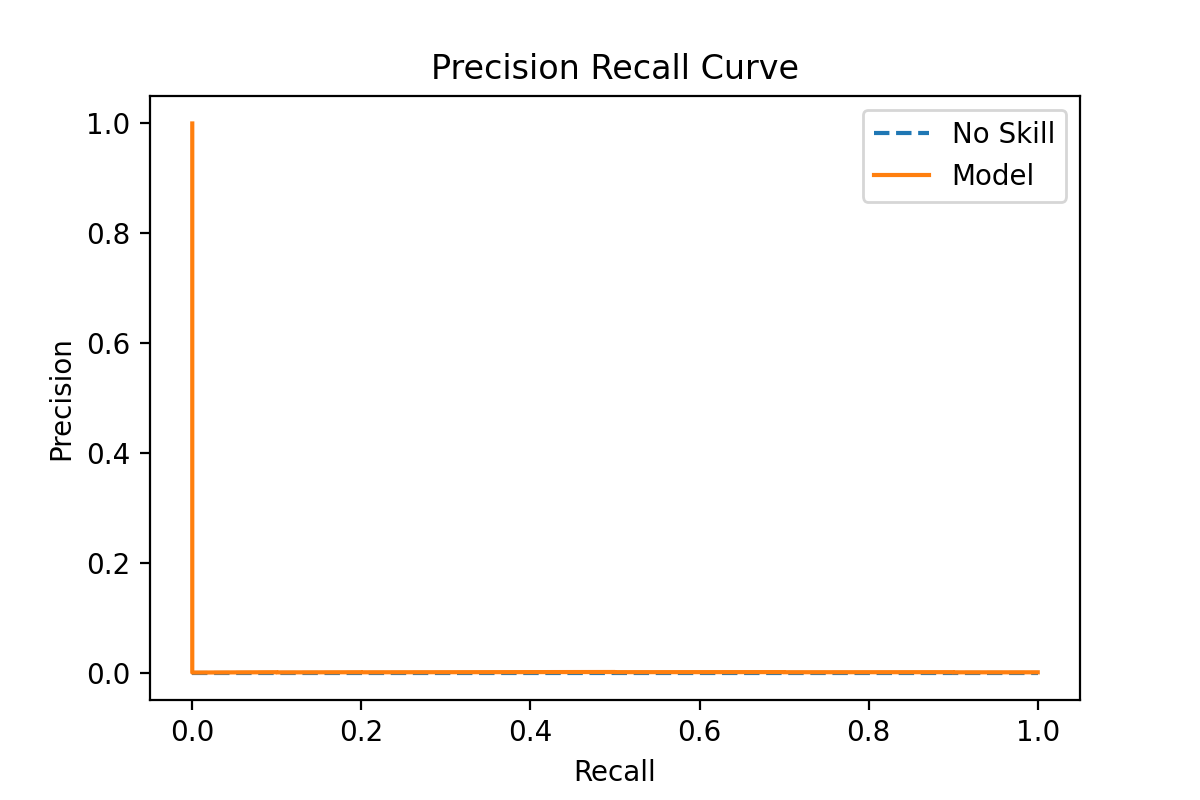
\includegraphics[width=\linewidth]{mlp-pr-low.png}
    \caption{PR Curve for TS2.}
  \end{minipage}
  \begin{minipage}{0.32\textwidth}
    \centering
    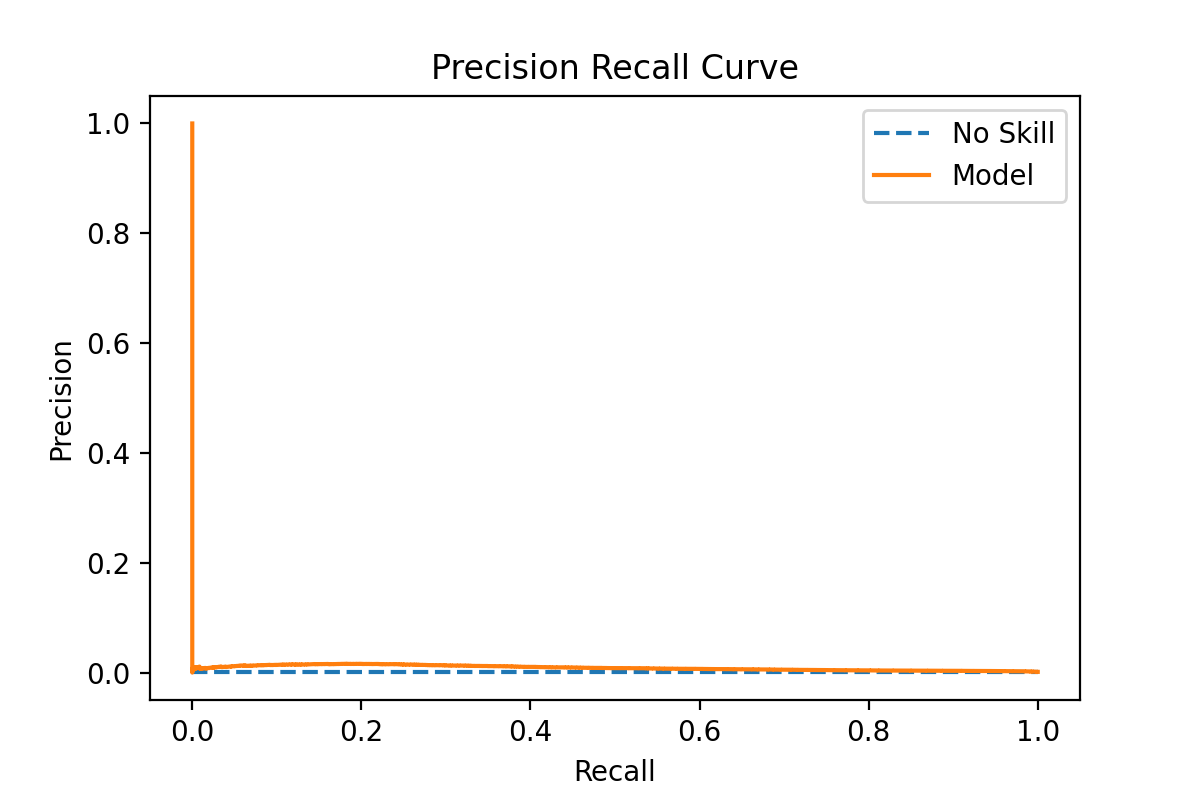
\includegraphics[width=\linewidth]{mlp-pr-medium.png}
    \caption{PR Curve for TS3.}
  \end{minipage}
  \begin{minipage}{0.32\textwidth}
    \centering
    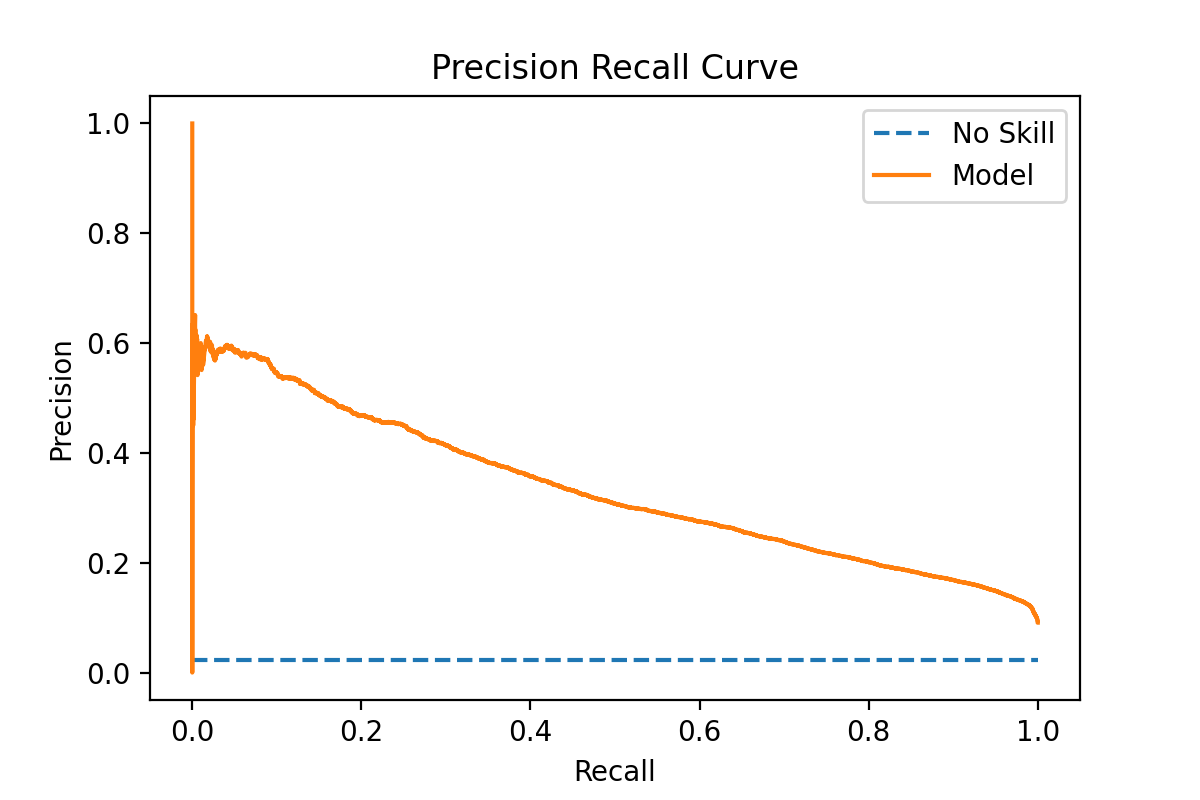
\includegraphics[width=\linewidth]{mlp-pr-high.png}
    \caption{PR Curve for TS4.}
  \end{minipage}
  \caption{PR Curves for MLP Test Datasets.}
  \label{fig:mlp-pr}
\end{figure}

Figure \ref{fig:mlp-cm} depict the confusion matrices for the various
test datasets. The confusion matrices highlight the strengths and
weaknesses of the model better than the ROC and PR curves. The model
has a very low number of FNs and FPs which is extremely valuable as
this ensures that the model does not miss hits from neutrino events
and also does not classify hits from noise sources incorrectly as hits
from neutrino events.

\begin{figure}[htb]
  \centering
  \begin{minipage}{0.49\textwidth}
    \centering
    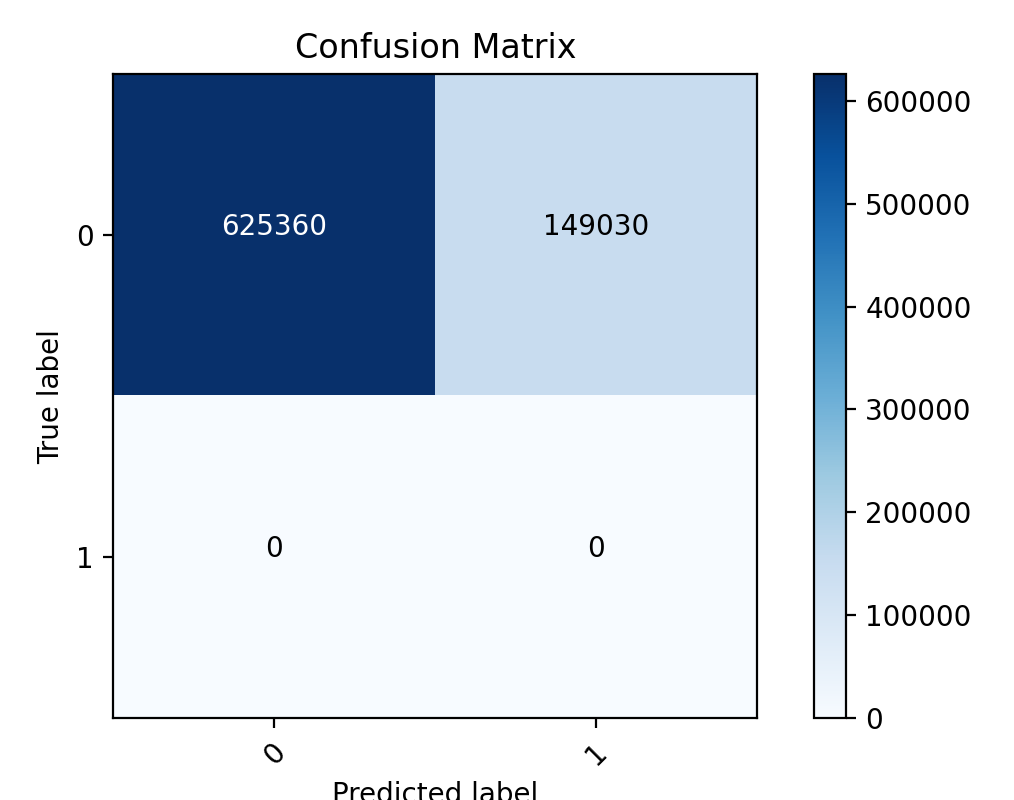
\includegraphics[width=\linewidth]{mlp-cm-no.png}
    \caption{Confusion Matrix for TS1.}
    \label{fig:mlp-cm-no}
  \end{minipage}
  \begin{minipage}{0.49\textwidth}
    \centering
    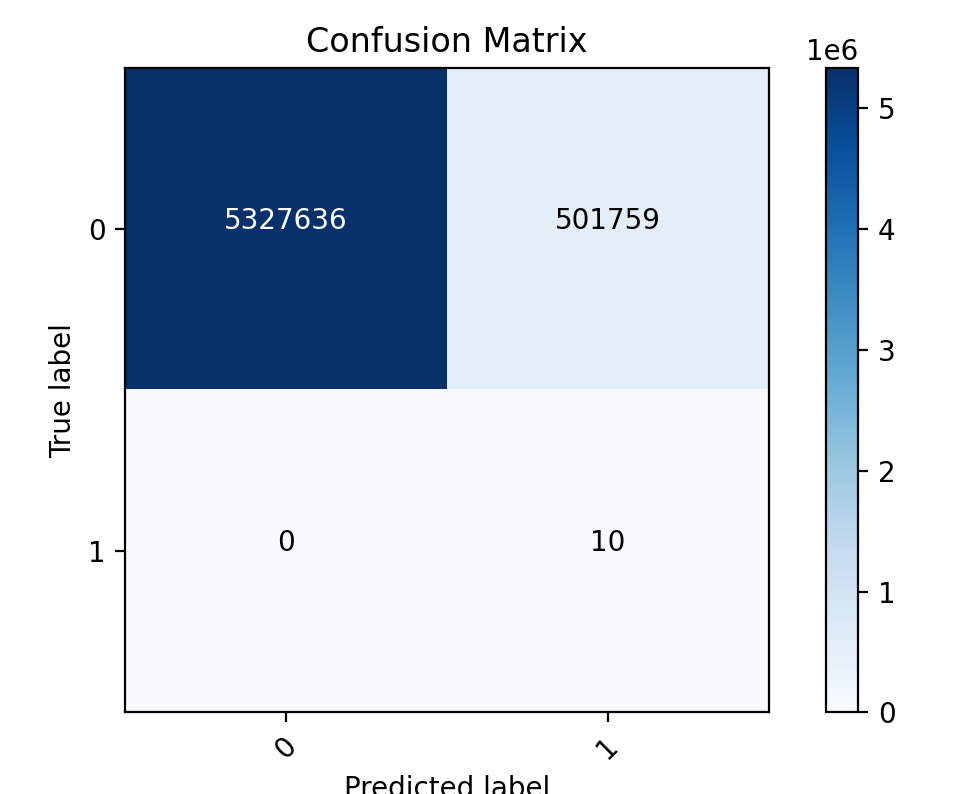
\includegraphics[width=\linewidth]{mlp-cm-low.png}
    \caption{Confusion Matrix for TS2.}
    \label{fig:mlp-cm-low}
  \end{minipage}
  \begin{minipage}{0.49\textwidth}
    \centering
    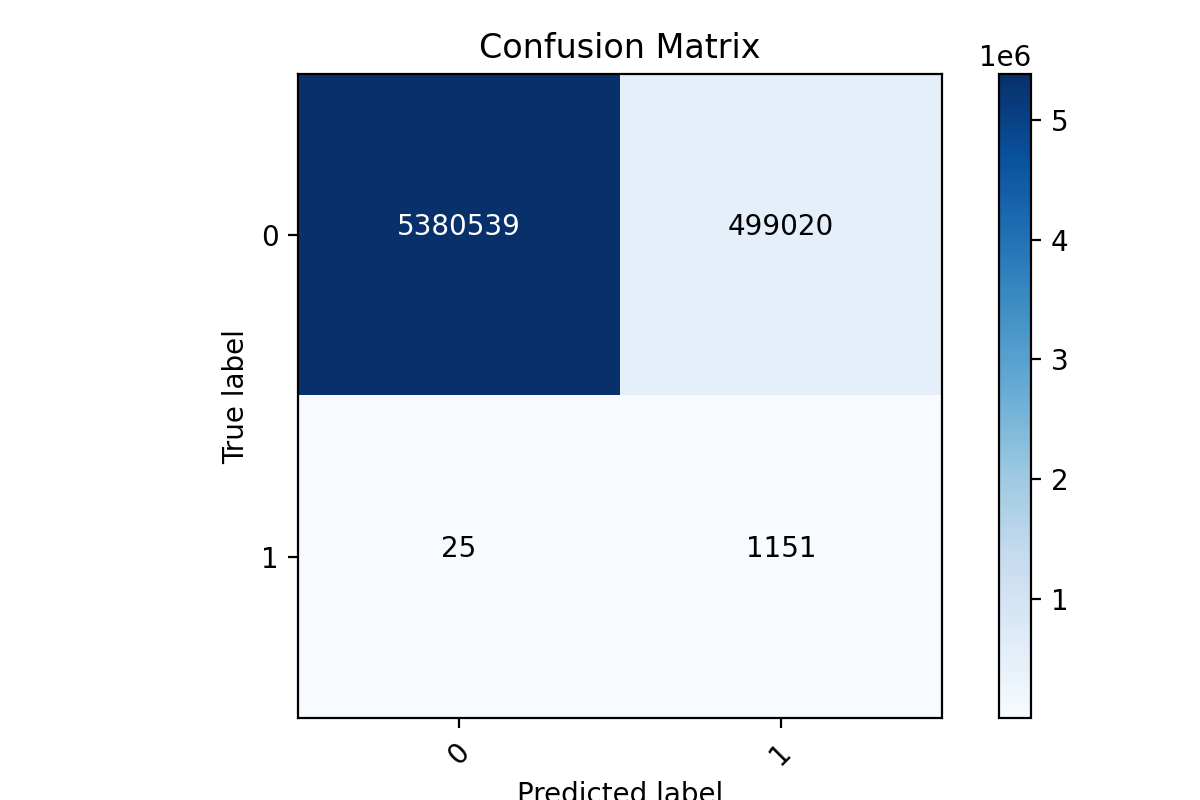
\includegraphics[width=\linewidth]{mlp-cm-medium.png}
    \caption{Confusion Matrix for TS3.}
    \label{fig:mlp-cm-medium}
  \end{minipage}
  \begin{minipage}{0.49\textwidth}
    \centering
    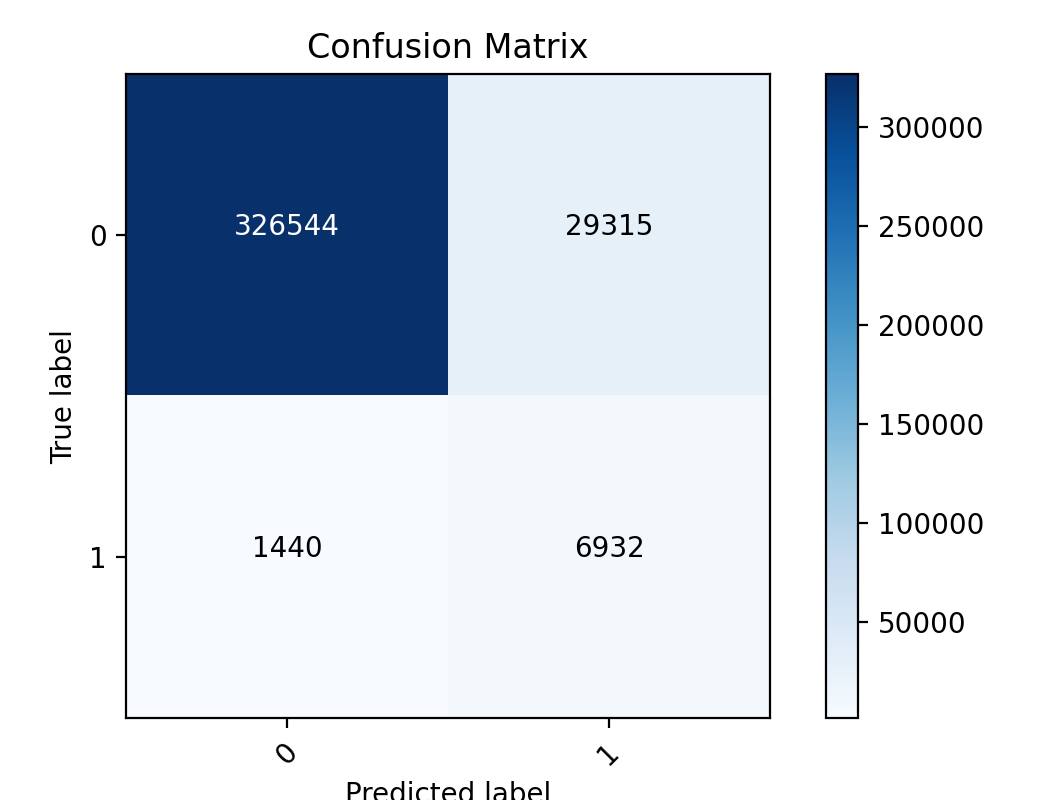
\includegraphics[width=\linewidth]{mlp-cm-high.png}
    \caption{Confusion Matrix for TS4.}
    \label{fig:mlp-cm-high}
  \end{minipage}
  \caption{Confusion Matrices of MLP Test Datasets.}
  \label{fig:mlp-cm}
\end{figure}

% ---------------------------------------------------------------------------
% ----------------------- end of thesis sub-document ------------------------
% ---------------------------------------------------------------------------
